\documentclass[fleqn,10pt]{wlscirep}
\usepackage[utf8]{inputenc}
\usepackage[T1]{fontenc}
\usepackage{lineno}
\linenumbers

\title{Insights into biotic and abiotic modulation of the ocean mesopelagic community}

\author[1,$\dag$]{Janaina Rigonato}
\author[2,$\dag$]{Marko Budinich}
\author[1,2]{...}
\author[1,*]{Olivier Jaillon}
\affil[1]{Genoscope, department, city, postcode, country}
\affil[2]{GO-SEE, department, Roscoff, postcode, country}

\affil[*]{corresponding author(s): Olivier Jaillon (corresponding.author@email.example)}

\affil[$\dag$]{these authors contributed equally to this work}


\begin{abstract}
Extended Abstract Version
\end{abstract}

\begin{document}
\flushbottom
\maketitle
%  Click the title above to edit the author information and abstract

\thispagestyle{empty}



\section*{Background \& Summary}

By definition the mesopelagic zone is commonly delimited between 200–1,000 m depth bellow the ocean surface. Also, the low incidence of light in the water column, limiting the photosynthetic metabolism, until its total absence, where hunting is no more realized by visual search can be considered the biological top-down limits to the mesopelagic layer, though also called twilight zone ((1)(Robinson et al., 2010).

Previous reports showed the stratification of the communities in water layers with taxonomy changing with depth, where the mesopelagic zone upholds a distinct assemblage  of dsDNA viruses ((2)Gregory et al 2019), giruses (HIRO paper), prokaryotes ((3,4)Sunagawa et al 2015, Salazar 2019) and eukaryotes ((5)Giner et al 2020). Also, differently from epipelagic, the mesopelagic diversity does not follow the latitudinal diversity gradient trends from poles increasing towards the equator ((6)Ibarbalz et al 2019).

Another characteristic that attracted our attention to mesopelagic region is the occurrence of zones with low concentration of oxygen called OMZ. There are indications that these zones are increasing in volume in the oceans, so understanding the communities dynamic in these regions can help to predict possible impacts faced by global warming changes.

The present study takes advantage of the Tara Oceans expedition large-scale survey conducted in different water layers and in a systematic sampling protocol, spanning from viruses to small eukaryotes size fractions, to investigate the mesopelagic complex biome. We capitalized the produced data together with the water physico-chemical properties and ocean geography to explore the differences on mesopelagic community compared to upper layers structuring. We also investigate possible effects in water deoxygenation on mesopelagic community, by means of comparison of oxygen minimum zones communities with that from well oxygenated waters. This work expands our knowledge about the web of relationship forming mesopelagic ecosystem in a wide geographically scale.

\section*{Results}

In this study, we analyzed the community of 32 stations that were sampled in epipelagic and mesopelagic waters, including 13 samples characterized by low concentration of oxygen (OMZ). Our data set was composed by NCDLV viruses (from hereafter named as giruses), two dsDNA-viruses families podoviridae and mioviridae (from hereafter named as viruses), 16S rRNA Mitags-prokaryotes and V9 18S rRNA pico-eukaryotes (0.8-5/0.8-3 um).

\textit{As previously reported, we observed the epi/mesopelagic community stratification according to water column depth for dsDNA-viruses, gyruses, prokaryotes, and pico-eukaryotes.}  (Figure \ref{fig:nmds}).


\textbf{Maybe this paragraph is not useful anymore, all this info is already published}


\begin{figure}[ht]
    \centering
    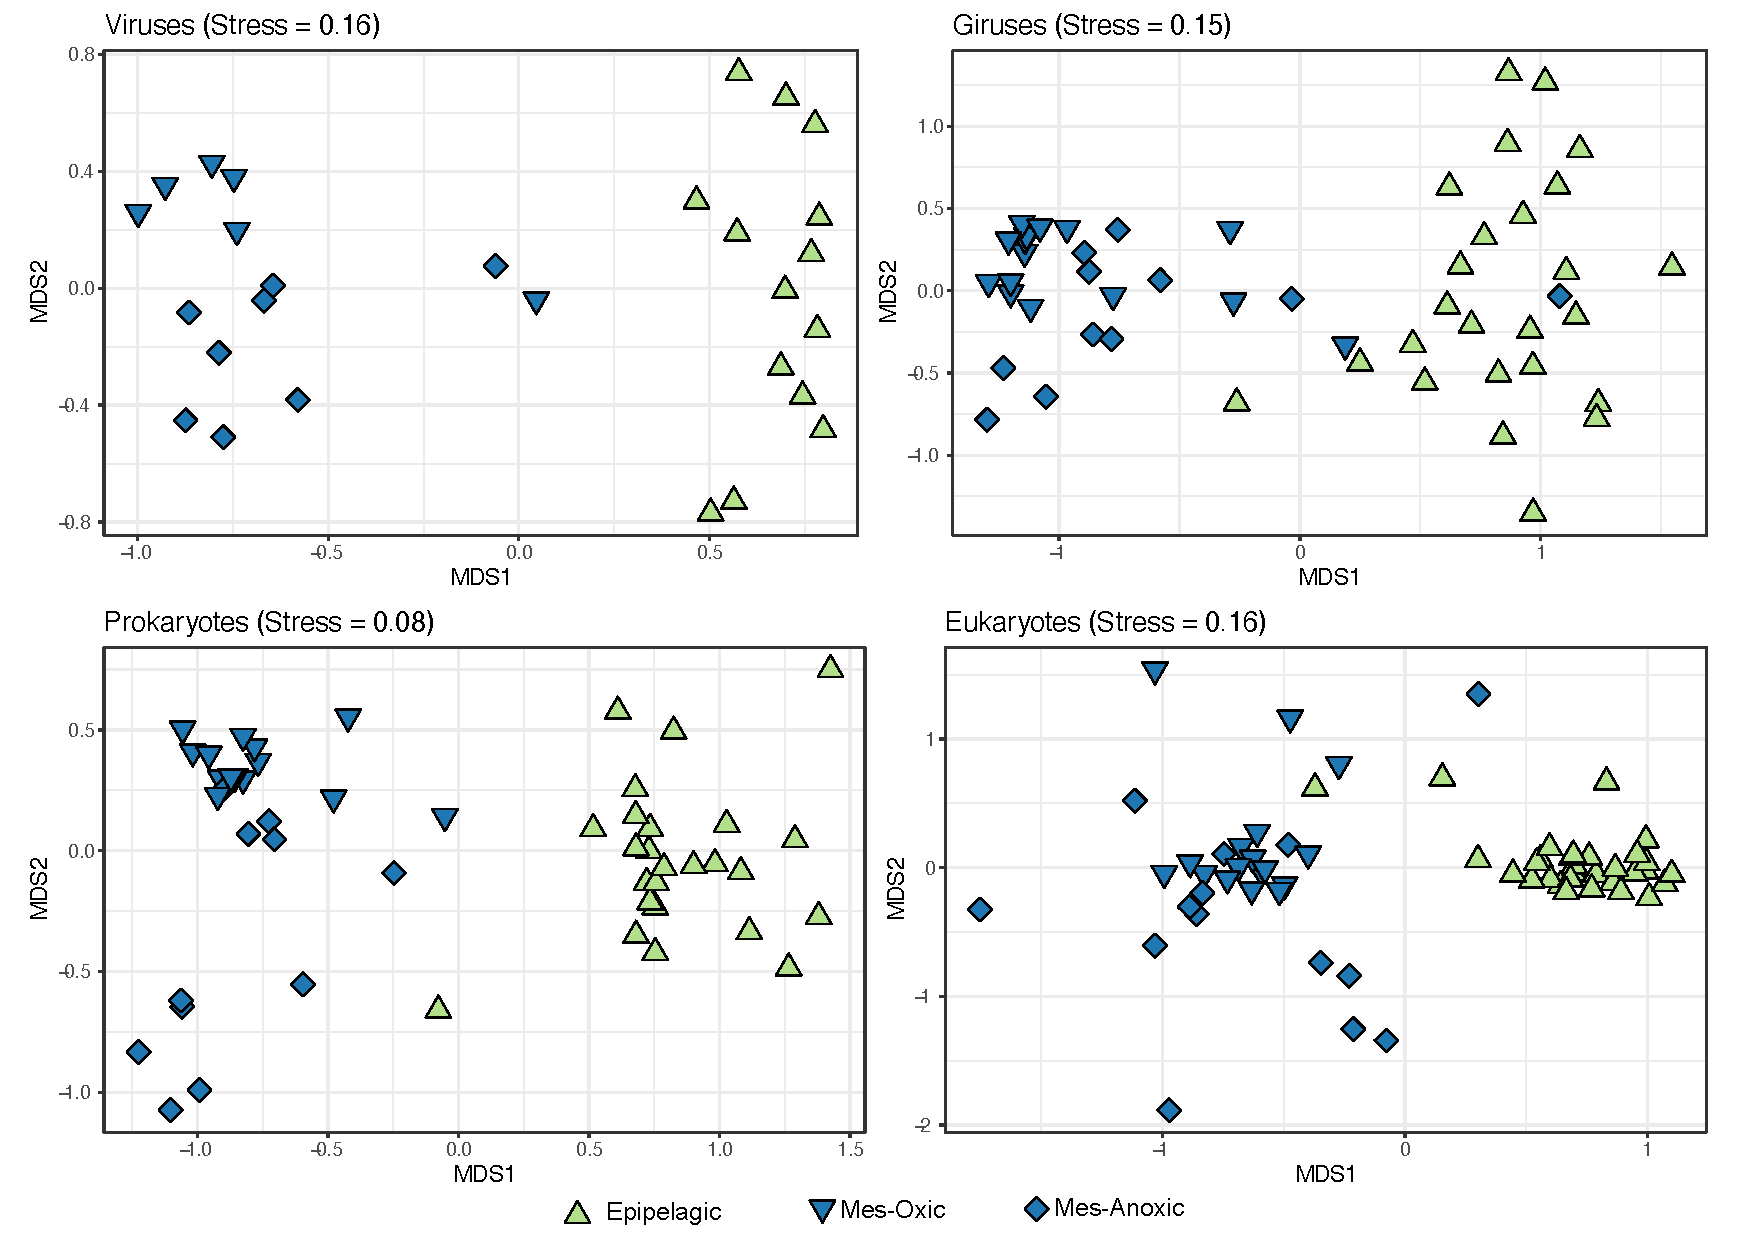
\includegraphics[scale=0.5]{images/nmds_used_SF_to_print.pdf}
    \caption{NMDS (k=2) plot of Samples for each domain}
    \label{fig:nmds}
\end{figure}

Our first goal was to understand how much of the mesopelagic planktonic variation can be explained by environmental variables currently indicated as important in oceanography, such as temperature, oxygen, salinity, NO3, chlorophyll-a and particle flux (UVP). Also 

We compared mesopelagic sampling sites by means of their physico-chemical properties, using Euclidian distance. We observed a slightly but significant higher heterogeneity among mesopelagic sites than that observed for the same epipelagic stations (Figure \ref{fig:betadipersion})

\begin{figure}[ht]
    \centering
    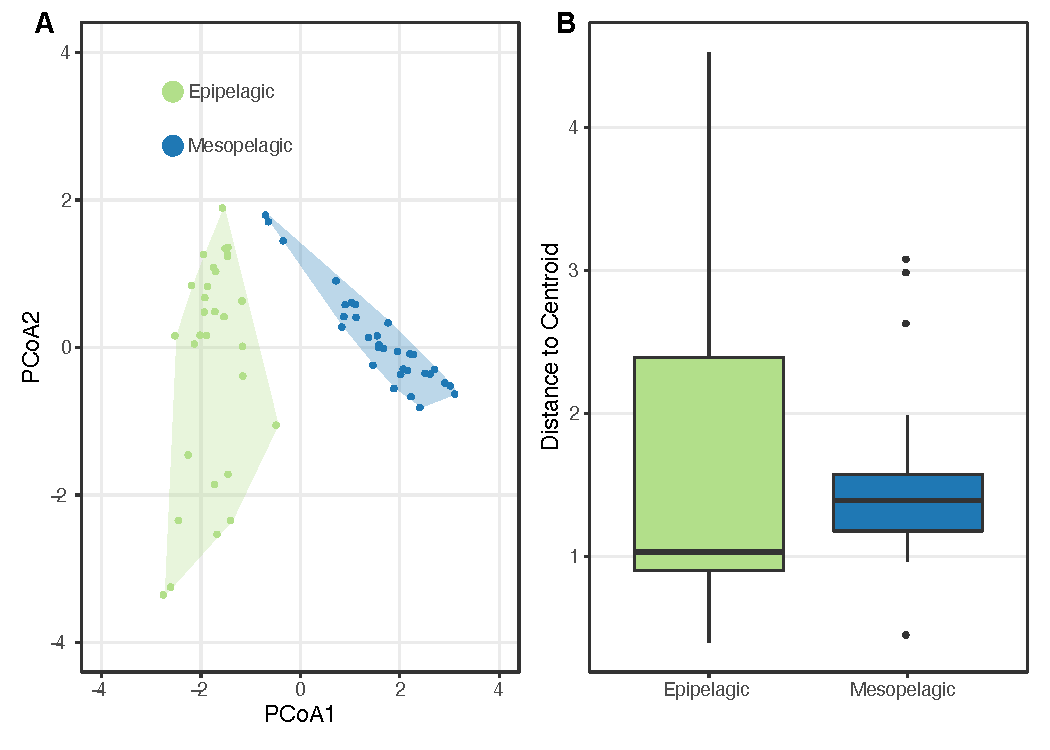
\includegraphics[scale=0.5]{images/betadisp_diganose_to_print.pdf}
    \caption{Betadispertion Analysis. A) First two axes of PCoA. B) Dispersion of distances from Samples to Centroids.}
    \label{fig:betadipersion}
\end{figure}

Our work has led us to conclude that similarly to epipelagic the mesopelagic community is organized according to niche/deterministic ecological models (table sup2), and the great majority of both epi and mesopelagic samples better fitted the lognormal model, this kind of relationship appears often in communities. One theory is that species are affected by many factors including environment and biotic competitive interactions (ref). 

In these words, we could observe that the environment can explain a small fraction of the communities variance for both layers (figure 1). The exception was verified to the virus assemblage which about 62\% of epipelagic variation and 70\% of mesopelagic variation can be explained by the environmental factors included in the analysis (Figure ?). 

But, differently to epipelagic community, which is mainly governed by temperature and oxygen gradients as previously reported ((2,3,5–7) Sunagawa 2015,Gregory 2019, Ibarbalz 2019, Giner 2020, Ghiglione 2012), we could not identify common environmental predictors structuring all the mesopelagic assemblies, but few different variables appeared as significant for different groups (table Sup3). This shows that the environmental factors tested are equally important in structuring mesopelagic community. Probably the lower spectra of the physicochemical variables in mesopelagic layer and its intrinsic heterogeneity given by deep currents, shear zones, intertidal tides and eddies, favor a patchy diversification in the mesopelagic community adaptation/acclimation. To further investigate this hypothesis, we identified the occurrence of nine different water masses (fig sup 3) at the mesopelagic depth sampled. All the assemblies studied (viruses, giruses, prokaryote and eukaryotes) This is reinforced by the fact that the mesopelagic community variation is better explained by the different water masses occurrences (figure xx table).

Specifically, the oxygen in the mesopelagic layer was the main driver to explain the viruses and prokaryotes variation, as previously reported (OMZ prok papers). On the other hand, even though we observed in the ordination plots  the distinction of OMZ and Oxic stations also for giruses and eukaryotes groups (Figure \ref{fig:cca_OS}), we cannot disentangle the effect of the oxygen from the others variables included in the analyses (table sup 3). Showing that these assemblies are equally affected by all the predictors evaluated, coping a larger environmental gradient that maximizes their niche-space partitioning.

\begin{figure}[ht]
    \centering
    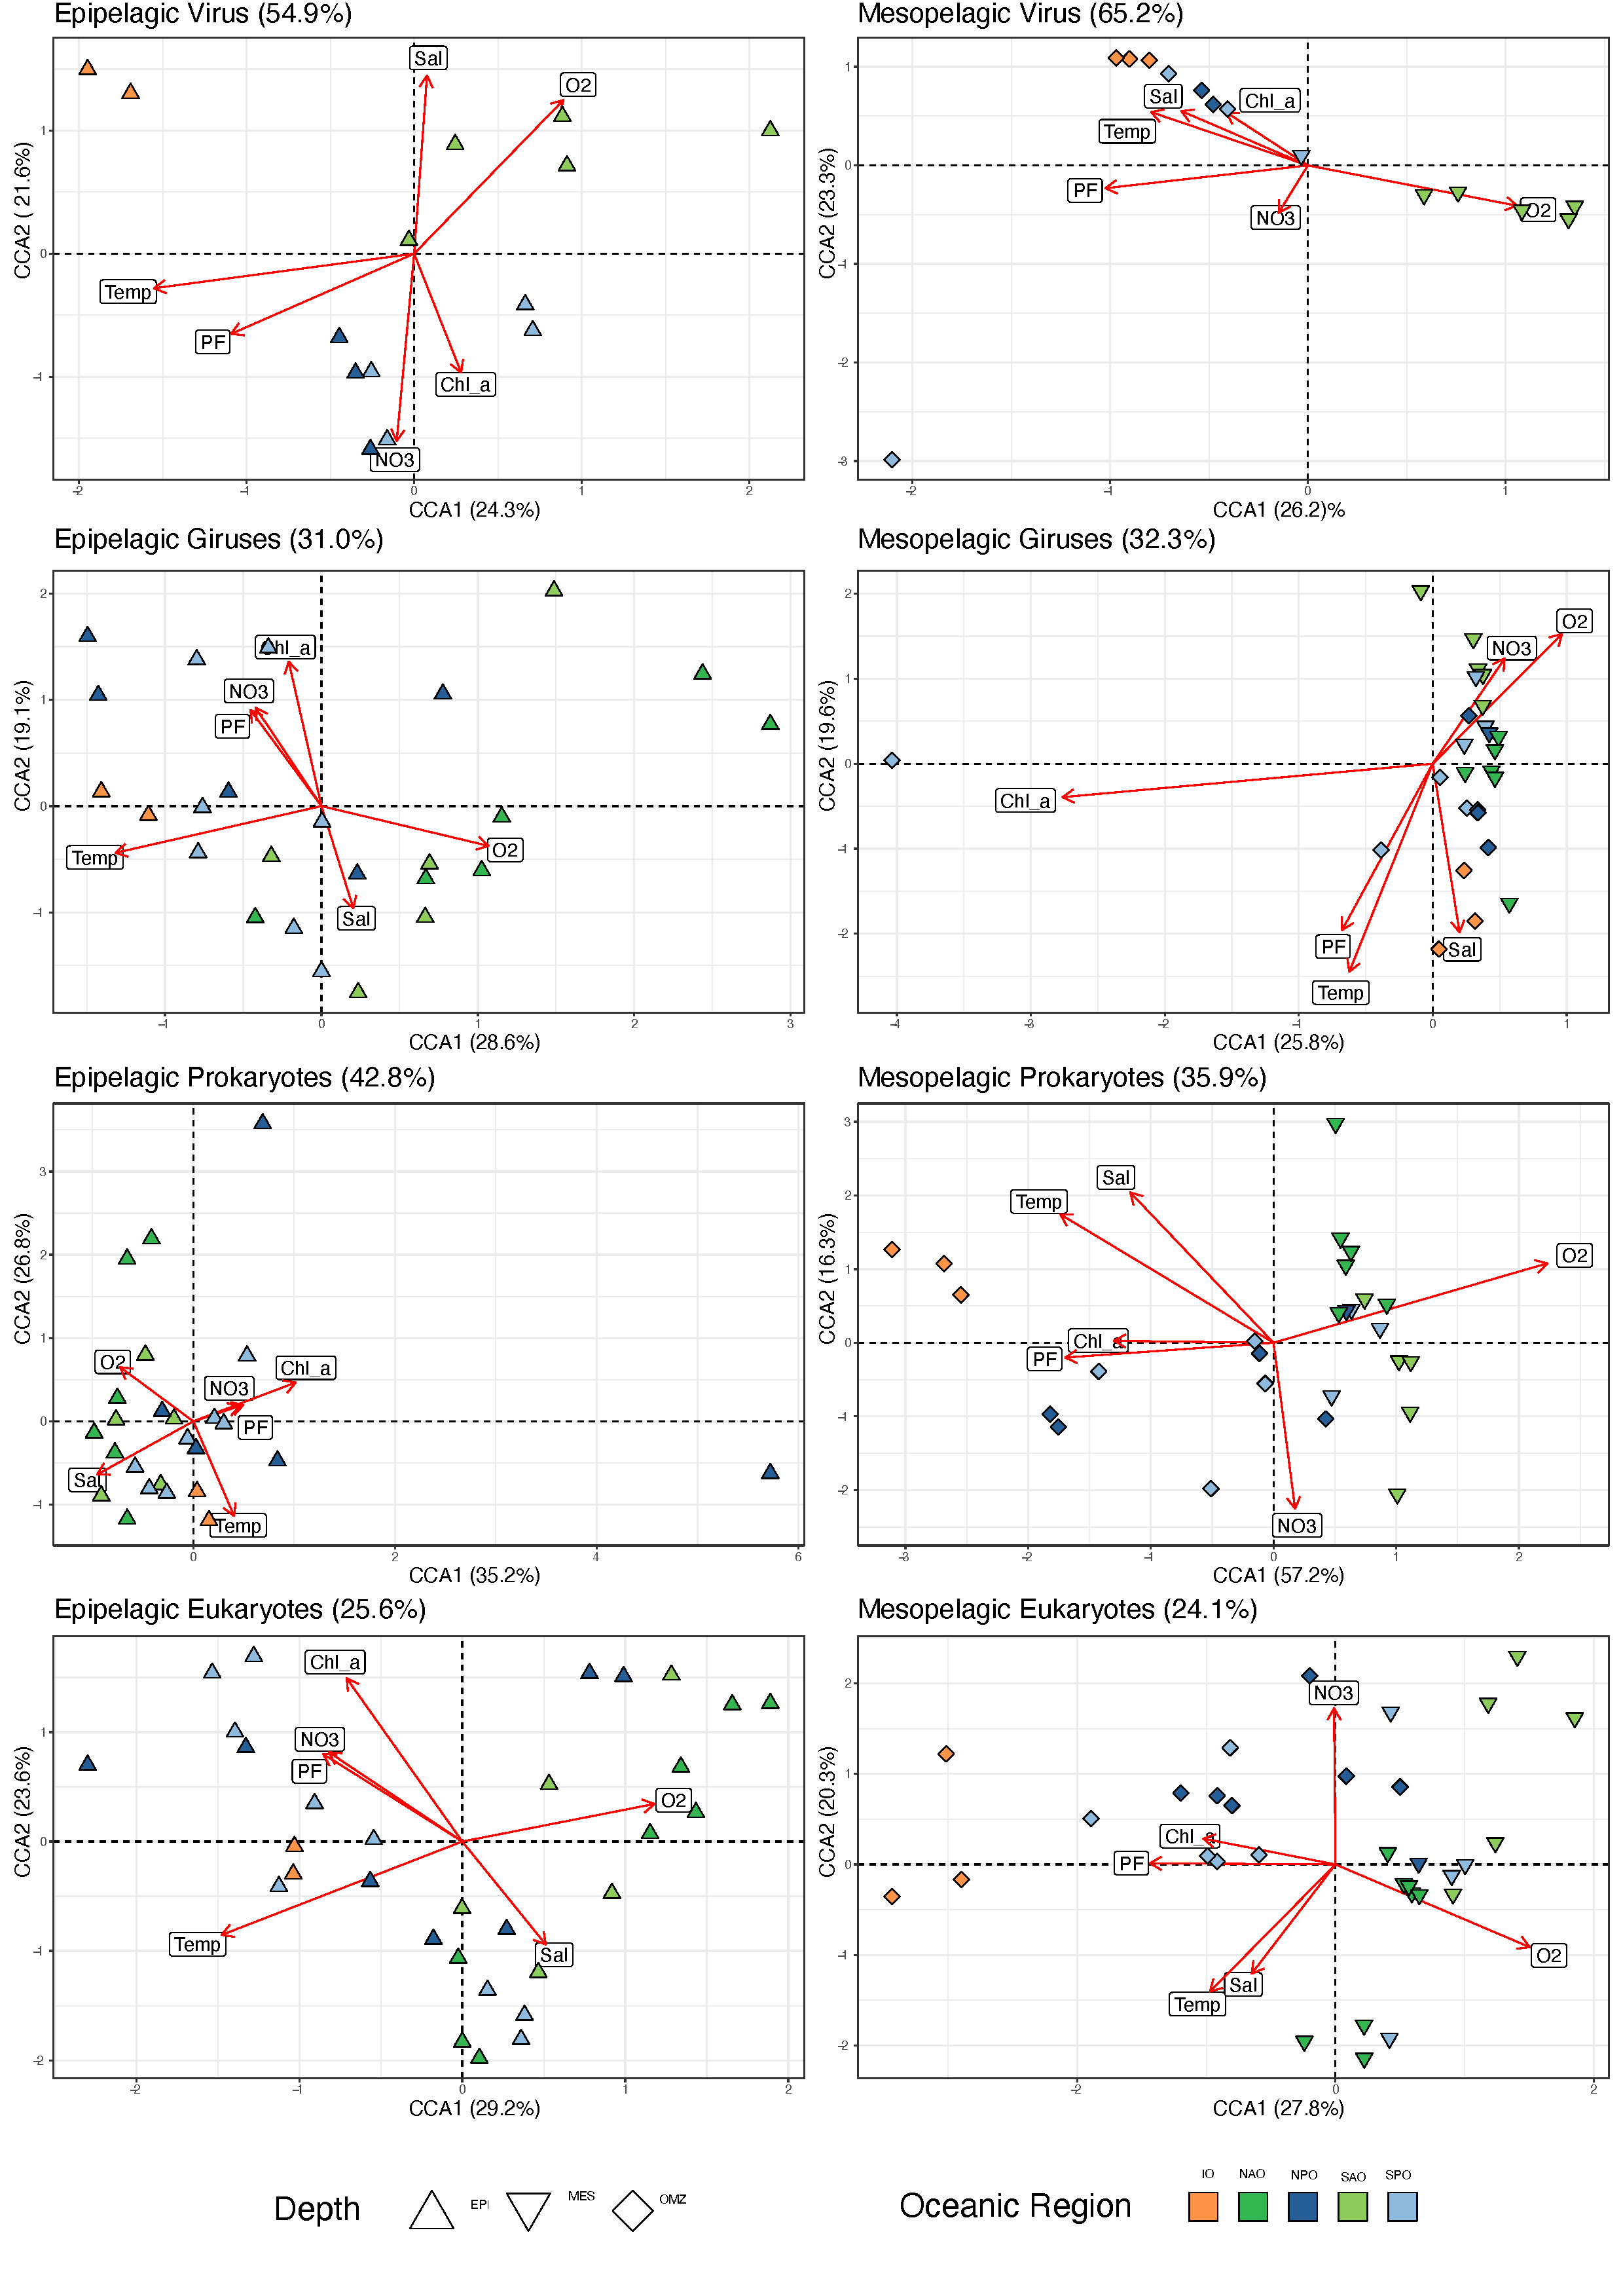
\includegraphics[scale=0.4]{images/custom_cca_plot_hellinger_no_bathy_labels_OS_regions_colors_to_print.pdf}
    \caption{CCA per Kingdom domain. IO: Indean Ocean, ...}
    \label{fig:cca_OS}
\end{figure}



%\subsection*{Subsection}
%
%Example text under a subsection. Bulleted lists may be used where appropriate, e.g.
%
%\begin{itemize}
%\item First item
%\item Second item
%\end{itemize}
%
%\subsubsection*{Third-level section}
% 
%Topical subheadings are allowed.
%
%\section*{Data Records}
%
%The Data Records section should be used to explain each data record associated with this work, including the repository where this information is stored, and to provide an overview of the data files and their formats. Each external data record should be cited numerically in the text of this section, for example \cite{Hao:gidmaps:2014}, and included in the main reference list as described below. A data citation should also be placed in the subsection of the Methods containing the data-collection or analytical procedure(s) used to derive the corresponding record. Providing a direct link to the dataset may also be helpful to readers (\hyperlink{https://doi.org/10.6084/m9.figshare.853801}{https://doi.org/10.6084/m9.figshare.853801}).
%
%Tables should be used to support the data records, and should clearly indicate the samples and subjects (study inputs), their provenance, and the experimental manipulations performed on each (please see 'Tables' below). They should also specify the data output resulting from each data-collection or analytical step, should these form part of the archived record.
%
%\section*{Technical Validation}
%
%This section presents any experiments or analyses that are needed to support the technical quality of the dataset. This section may be supported by figures and tables, as needed. This is a required section; authors must present information justifying the reliability of their data.
%
%\section*{Usage Notes}
%
%The Usage Notes should contain brief instructions to assist other researchers with reuse of the data. This may include discussion of software packages that are suitable for analysing the assay data files, suggested downstream processing steps (e.g. normalization, etc.), or tips for integrating or comparing the data records with other datasets. Authors are encouraged to provide code, programs or data-processing workflows if they may help others understand or use the data. Please see our code availability policy for advice on supplying custom code alongside Data Descriptor manuscripts.
%
%For studies involving privacy or safety controls on public access to the data, this section should describe in detail these controls, including how authors can apply to access the data, what criteria will be used to determine who may access the data, and any limitations on data use. 
%
%\section*{Code availability}
%
%For all studies using custom code in the generation or processing of datasets, a statement must be included under the heading "Code availability", indicating whether and how the code can be accessed, including any restrictions to access. This section should also include information on the versions of any software used, if relevant, and any specific variables or parameters used to generate, test, or process the current dataset. 


\bibliography{sample}

\noindent LaTeX formats citations and references automatically using the bibliography records in your .bib file, which you can edit via the project menu. Use the cite command for an inline citation, e.g. \cite{Kaufman2020, Figueredo:2009dg, Babichev2002, behringer2014manipulating}. For data citations of datasets uploaded to e.g. \emph{figshare}, please use the \verb|howpublished| option in the bib entry to specify the platform and the link, as in the \verb|Hao:gidmaps:2014| example in the sample bibliography file. For journal articles, DOIs should be included for works in press that do not yet have volume or page numbers. For other journal articles, DOIs should be included uniformly for all articles or not at all. We recommend that you encode all DOIs in your bibtex database as full URLs, e.g. https://doi.org/10.1007/s12110-009-9068-2.

\section*{Acknowledgements} (not compulsory)

Acknowledgements should be brief, and should not include thanks to anonymous referees and editors, or effusive comments. Grant or contribution numbers may be acknowledged.

\section*{Author contributions statement}

Must include all authors, identified by initials, for example:
A.A. conceived the experiment(s), A.A. and B.A. conducted the experiment(s), C.A. and D.A. analysed the results. All authors reviewed the manuscript. 

\section*{Competing interests} (mandatory statement)

The corresponding author is responsible for providing a \href{https://www.nature.com/sdata/policies/editorial-and-publishing-policies#competing}{competing interests statement} on behalf of all authors of the paper. This statement must be included in the submitted article file.

\section*{Figures \& Tables}


\begin{table}[ht]
\centering
\begin{tabular}{|l|l|l|}
\hline
Condition & n & p \\
\hline
A & 5 & 0.1 \\
\hline
B & 10 & 0.01 \\
\hline
\end{tabular}
\caption{\label{tab:example}Legend (350 words max). Example legend text.}
\end{table}

\end{document}